% !TeX root = ../summary-syssec.tex

\section{Side Channel Attacks}
\subsection{Introduction}
Security proofs based on models of system and attacker. Most models do not take
into account the implementation and how it interacts with the environment.

Examples:
\begin{itemize}
  \item Faulty Output (Glitch)
  \item Power Consumption
  \item EM Emissions
  \item Heat
  \item Timing
  \item Design Details
  \item Sound
  \item Data Coupling
\end{itemize}

\begin{description}
  \item[Simple] computation only depends upon the key.
  \item[Differential] computation depends upon both the input and the key.
\end{description}

\subsection{Timing Cryptanalysis of RSA}
\begin{enumerate}
  \item Execution time depends on the key
  \item Can be measured for different inputs
\end{enumerate}


\subsubsection{Square-And-Multiply}

\begin{itemize}
  \item Key-dependent Branching
  \item Attacker observes how many 1 are in the key
\end{itemize}
Greatly reduces the search space for the secret key, but still huge...

\subsubsection{Montgomery multiplication}
Multiplication the execution time depends on \textbf{input and key}.

Attack main idea:
\begin{itemize}
  \item Try large number of different messages and leverage average.
  \item Simulate execution up to round $i$ (using known key bits)
  \item Try many messages, measure execution time
\end{itemize}

\subsubsection{Protecting}
\begin{itemize}
  \item Change implementation s.t. it is not time dependent.
  \item Generic protection is hard.
  \item Performance Penalty
\end{itemize}


\subsection{Cache Attacks}
\subsubsection{Prime+Probe}
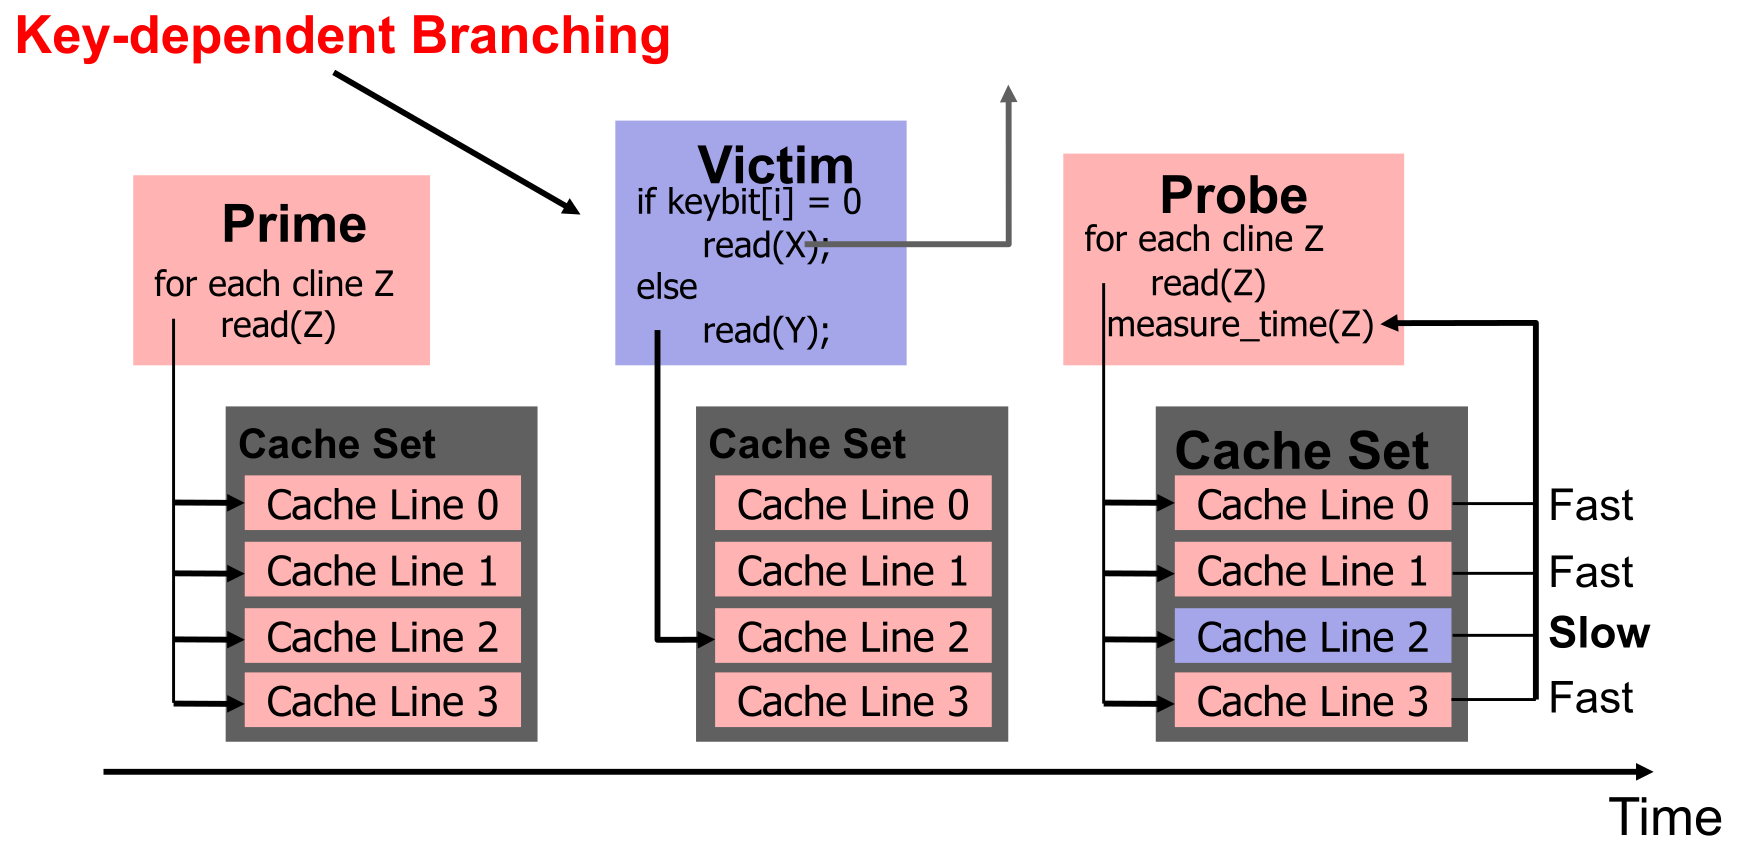
\includegraphics[width=\columnwidth]{sidechannel-prime-probe.png}
\subsubsection{Variants}
\begin{enumerate}
  \item \textbf{Data access} depends on secret data: Data access patterns
    in the cache leak information about the secret
  \item \textbf{Control flow} depends on secret data: Code access
    patterns in the cache leak information about the secret
\end{enumerate}
\subsubsection{Cache Timing Attack on AES}
During the execution of AES secret key is used to
index arrays (S-boxes). The time to lookup an array element depends
on whether this element of the S-box has partially or entirely been loaded into the
cache. Measuring the timing differences for these lookups allows the attacker to draw
conclusions about the key.

Most CPUs have special AES hardware  $\Rightarrow$ not vulnerable.
\subsubsection{Protecting}
\begin{itemize}
  \item \textbf{Basic principle:}
    Try to eliminate secret-dependent cache access patterns
  \item Specific defenses exist, but eliminating all secret-dependent
    branching (code and data) is difficult and expensive…
\end{itemize}

\subsection{Power Analysis Attacks}
Mainly used on Smartcards, RFID chips, Sensor Nodes
\begin{itemize}
  \item The attacker needs to have physical access
  \item Measures the consumed power during  operation
\end{itemize}
Square-and-multy in RSA is vulnerable through simple power analysis:
\subsubsection{Protection}
Goal: Elimination or significant reduction of the correlation between
\begin{itemize}
	\item Random change of power consumption in time
	\item Noise generator
	\item Physical shielding
	\item Software balancing
	\item Hardware balancing
\end{itemize}

\subsection{Acoustic Attacks}
\begin{itemize}
	\item High-frequency sounds caused by vibration of
electronic components
\item \textbf{Different keys cause different sounds}
  \item Can extract RSA keys based on sound
\end{itemize}
